%% content.tex
%%

%% ===========================
\chapter{Systemanalyse}
\label{ch:Systemanalyse}
%% ===========================

Zu Beginn der Arbeiten wird eine Systemanalyse zur Ermittlung des Ist- und Soll-Zustandes durchgeführt. Nach \cite{SWB-380277719} versteht man darunter das Beschreiben der vorhandenen und zukünftigen Systeme. Im Rahmen der Analyse ist die Kontextabgrenzung eines der wichtigsten Bestandteile. Dabei wird eine Abgrenzung zwischen dem Umfang und der Umgebung des Systems vorgenommen. Zuerst wird in Abschnitt \ref{ch:Systemanalyse:sec:genesisWorld} eine Ist-Analyse durchgeführt. In Abschnitt \ref{ch:Systemanalyse:sec:Anforderungsanalyse} wird auf die Anforderungen, die an das System gestellt werden eingegangen. Aufbauend auf den Anforderungen werden in Abschnitt \ref{ch:Systemanalyse:sec:Information}, die für die Umsetzung relevanten Daten, ermittelt. 

%% ===========================
\section{CAS genesisWorld}
\label{ch:Systemanalyse:sec:genesisWorld}
%% ===========================

CAS genesisWorld ist eine Software, die Organisation und Zusammenarbeit in Kundenbeziehungen und zwischen Kollegen steigern soll. Alle Informationen bzw. Daten werden in CAS genesisWorld zentral gespeichert und sind so für alle verfügbar. Welche Daten ein Anwender sieht, hängt von seinen Rechten und Einstellungen ab. Die Daten, d. h. Termine, Aufgaben, Adressen, Dokumente usw. werden in CAS genesisWorld von den Nutzern gepflegt und aktuell gehalten. Darüber hinaus lassen sich wie in Abbildung \ref{picGwCon} dargestellt, alle Daten beliebig miteinander verknüpfen. So werden zusätzliche Zusammenhänge deutlich und der Informationsgehalt erhöht sich. Ein Besprechungstermin lässt sich beispielsweise mit den Adressen, der Teilnehmer und dem Dokument der Tagesordnung verknüpfen.

\begin{figure}[H]
	\centering
  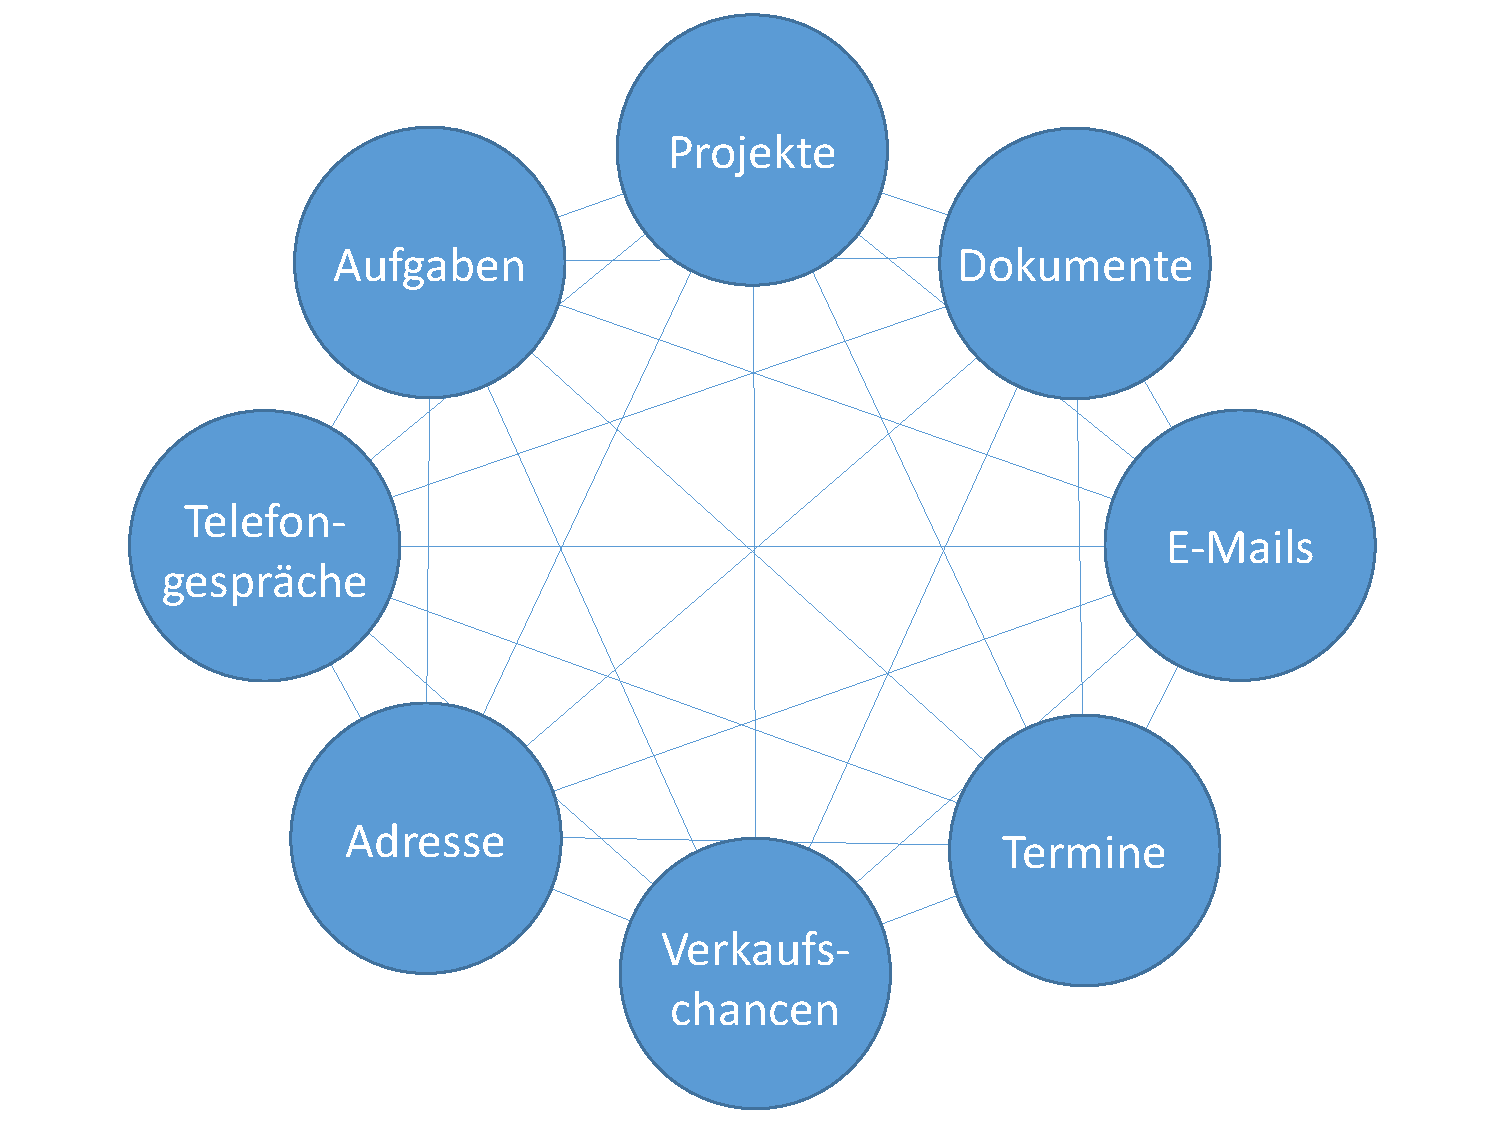
\includegraphics[width=0.5\textwidth, width=0.5\textwidth]{pics/CAS_connections.pdf}
	\caption{Schematische Darstellung der potenziellen Verknüpfungen}
	\label{picGwCon}
\end{figure}

%% ===========================
\subsection{Architektur}
%% ===========================

Die N-Tier-Architektur von CAS genesisWorld, lässt sich in drei wesentliche Bereiche gliedern:

\begin{itemize}
	\item Die Präsentationsclients umfassen alle Dienste, die Informationen in Bildschirm-Ansichten, dem Benutzern zur Verfügung stellen.
	\item Der Applikationsserver umfasst alle Dienste, die die Geschäftslogik kapseln, Änderungen protokollieren, Benutzerrechte prüfen und die aufbereiteten Informationen den Präsentationsdiensten zur Verfügung stellen.
	\item Die Datenbankschicht umfasst alle Dienste, die zur Datenhaltung selbst notwendig sind.
\end{itemize}


%% ===========================
\subsection{Präsentationsschicht \& Logikschicht}
%% ===========================

CAS genesisWorld Clients existieren in Form einer 32bit Windows Anwendung, sowie als Mobile Client in Android und iOS. Die Kommunikation der Mobile Clients mit CAS genesisWorld findet über das REST-Protokoll statt \cite{cas2013a}.

Die Funktionalität des CAS genesisWorld-Applikationsservers, wurde in Form von COM-Objekten implementiert. Damit stehen dessen Dienste auch Dritten zur Verfügung, die dadurch mit eigenen Applikationen die Informationen von CAS genesisWorld präsentieren oder weiterverarbeiten können. Als Basisdienste stehen der UserService und der DataService zu Verfügung. Für die Anmeldung und Rechteverwaltung ist der UserService zuständig. Der DataService hingegen, als zentraler Dienst für den Zugriff auf die CAS genesisWorld Daten. Die Schnittstelle des DataService wurde an Microsoft ADO angelehnt. Auf den Basisdiensten aufbauend existieren die Geschäftsdienste, in Form der Schnittstellen der BusinessServices. Diese bieten spezielle Funktionen zu den jeweiligen Anwendungsbereichen.

\begin{figure}[H]
	\centering
  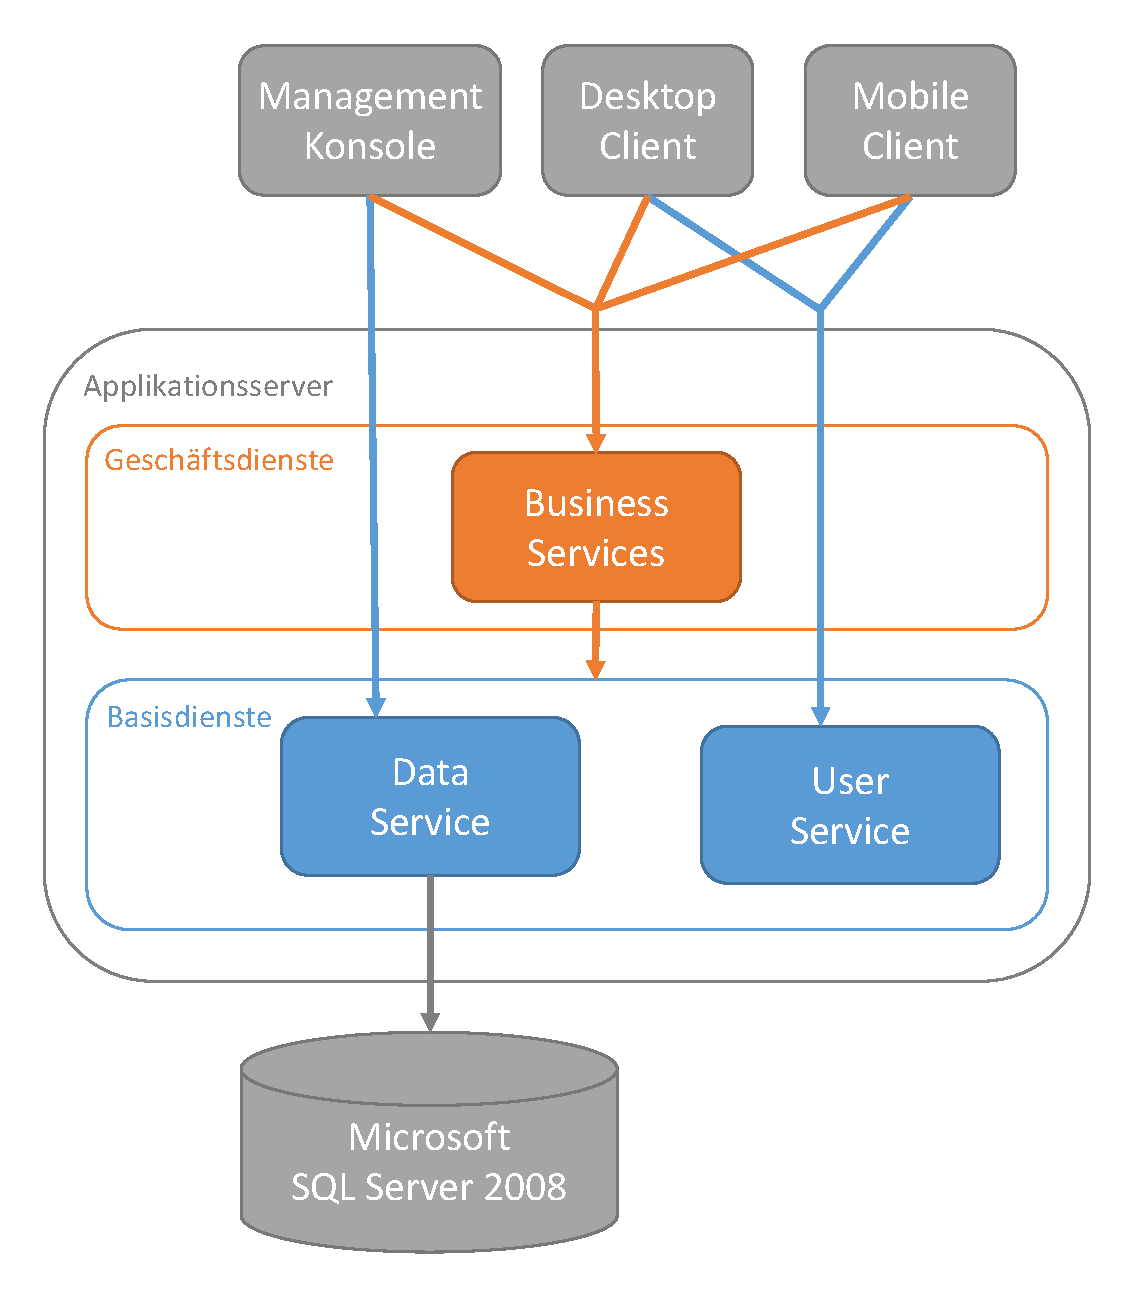
\includegraphics[width=0.6\textwidth, width=0.6\textwidth]{pics/GenesisWorld_Architektur.pdf}
	\caption{Schematische Darstellung der Architektur von CAS genesisWorld}
	\label{gw_Architektur}
\end{figure}

\paragraph{Server-SDK-PlugIns}

Die Server-SDK-PlugIns bieten die Möglichkeit, die Datenverarbeitung um eine eigene Logik zu erweitern oder zu modifizieren. 

Realisiert werden die PlugIns als COM-Objekte, die ein PlugIn-Interface namens \textit{IGWSDKDataPlugIn} implementieren. Das erstellte COM-Objekt wird im Server von CAS genesisWorld registriert. Der Server delegiert bei einer Datenoperation den Aufruf an die für den jeweiligen Datensatz-Typen registrierten PlugIns. In Abbildung \ref{gw_plugin} wird anhand eines Beispieles der Vorgang verdeutlicht.

\begin{figure}[H]
	\centering
  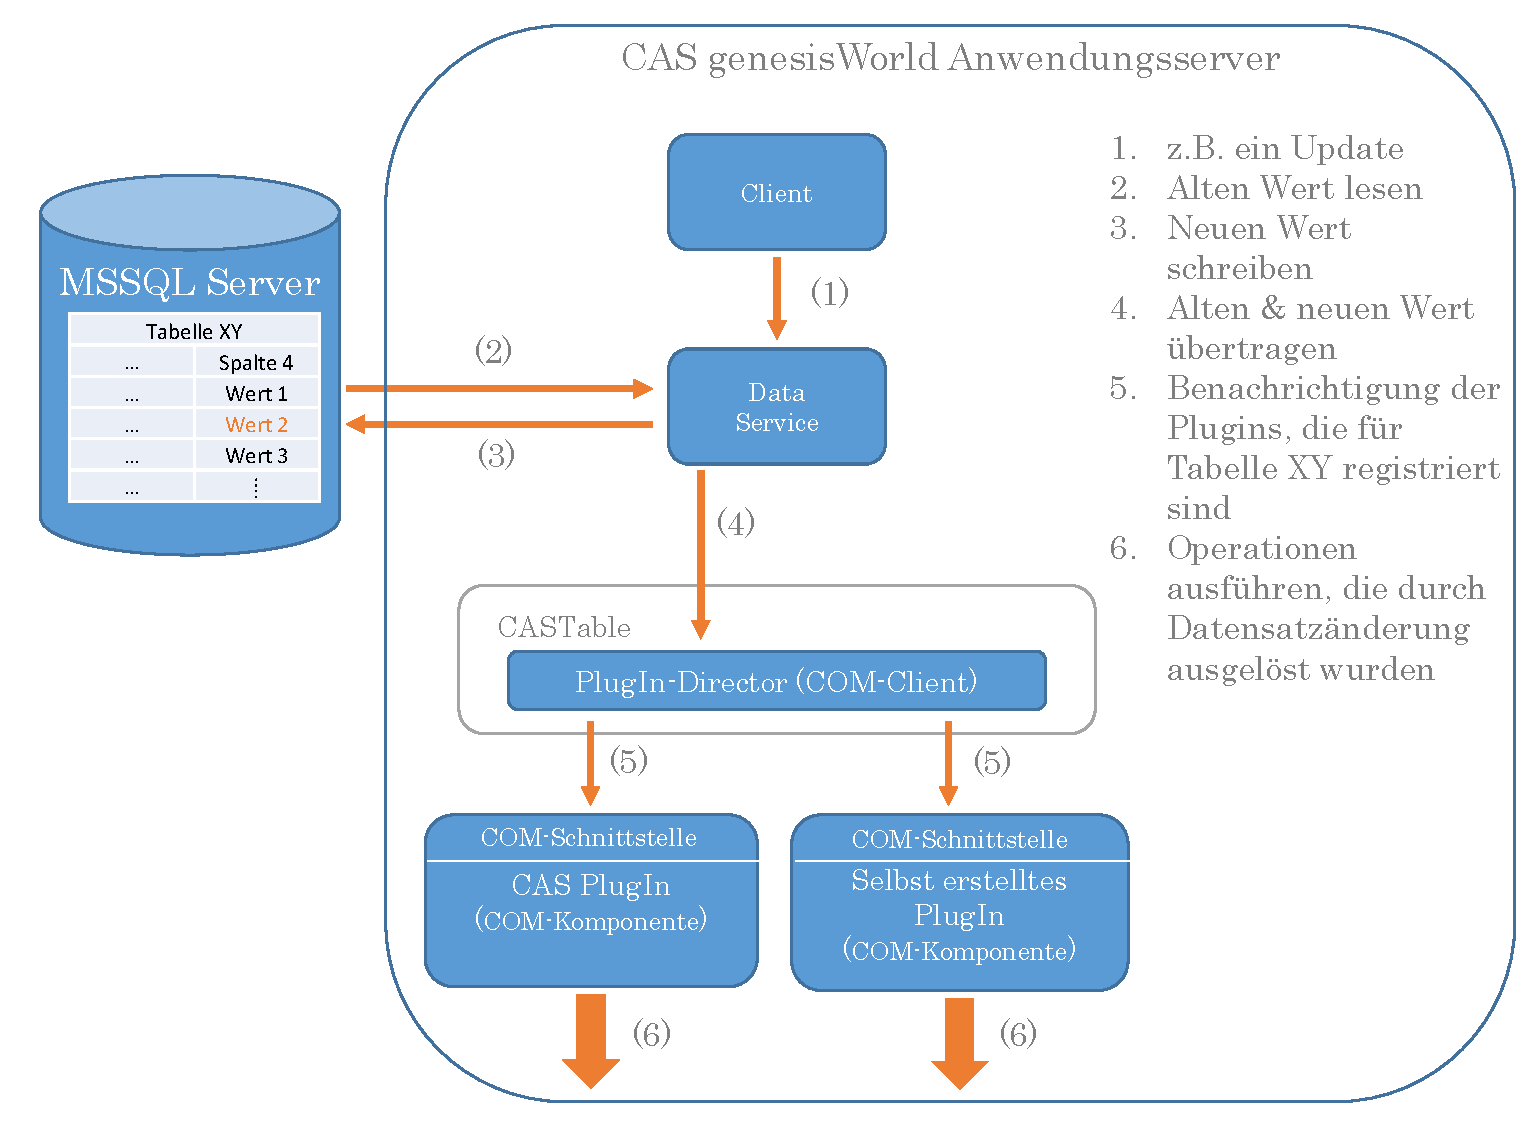
\includegraphics[width=1.0\textwidth, width=1.0\textwidth]{pics/analyse_plugins.pdf}
	\caption{Beispiel zur Benachrichtigung von PlugIns anhand eines Ablaufs bei einem Update}
	\label{gw_plugin}
\end{figure}

Im Allgemeinen stehen in den COM-Schnittstellen der PlugIns, jeweils alle Felder eines Datensatz-Typen zur Verfügung, sowie die individuelle Teilmenge der Felder mit neuen Werten. In den PlugIns besteht damit die Möglichkeit, alte bzw. neue Werte von Feldern zu untersuchen und zu vergleichen und auf das Ergebnis zu reagieren.

Die Werte-Teilmenge des aktuell verarbeiteten Datensatzes kann verändert, d.h. erweitert oder reduziert werden und die Werte selber sind änderbar. Darüber hinausgehend sind auch automatisierte Aktionen realisierbar, die weitere Datensätze betreffen. So könnten z.B. abhängig von den Eingangswerten einer neu angelegten Adresse, neue Aufgaben angelegt und mit Inhalt versehen werden. Einige automatische Datenoperationen von CAS genesisWorld werden über CAS PlugIns realisiert, die mit den SDK-PlugIns verwandt sind.

%% ===========================
\subsection{Datenhaltungsschicht}
\label{ch:Systemanalyse:sec:genesisWorld:subsec:db}
%% ===========================

Die Datenhaltungsschicht enthält einen Microsoft SQL Server 2008 (MSSQL). Der SQL Server ist ein relationales Datenbankmanagementsystem (RDBMS) von Microsoft, dass für den Einsatz im Konzern Umfeld konzipiert wurde. MSSQL verwendet T-SQL (Transact-SQL), eine Erweiterungen von Sybase und Microsoft, die mehrere Funktionen zum SQL-Standard hinzufügt \cite{tech2013}. Weiterhin unterstützt MSSQL standardisierte Datenbankschnittstellen, wie Open Database Connectivity (ODBC) und Java Database Connectivity (JDBC).
  
In den meisten relationalen Datenbanken werden Beziehungen über Primär-/ Fremdschlüsselbeziehungen hergestellt. In der CAS genesisWorld Datenbank werden nur Primärschlüssel eingesetzt. Die Beziehungen werden nicht wie sonst in mehreren Zwischentabellen realisiert, sondern in einer einzigen Tabelle, die \textit{RelationTable}. In Abbildung \ref{gw_2} ist ein Beispiel zu sehen.

\begin{figure}[ht]
	\centering
  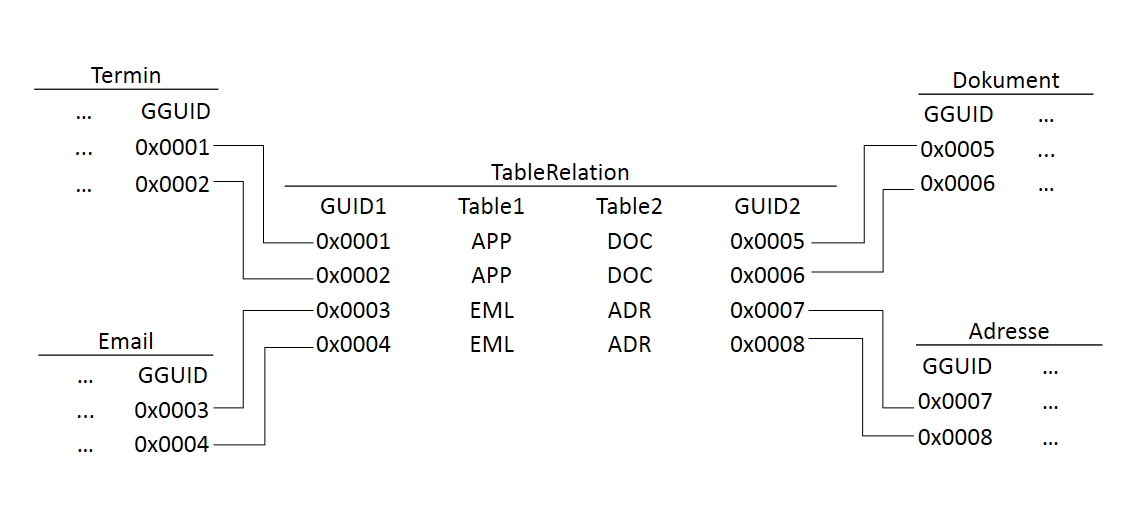
\includegraphics[width=0.9\textwidth, width=0.9\textwidth]{pics/gW_tablerealtion.png}
	\caption{Funktionsweise von RelationTable anhand eines Beispiels}
	\label{gw_2}
\end{figure}

Die Spalten \textit{GUID1} und \textit{GUID2} beinhalten die jeweiligen Primärschlüssel, der in Beziehung zu setzenden Tabellen. Als Zuordnungsmerkmal für die \textit{GGUID}s zu Ihren Tabellen, dienen die Spalten \textit{TableSign1} und \textit{TableSign2}, deren Werte Kürzel der Tabellennamen sind. Möglich wird die Verknüpfung verschiedener Tabellen, durch einen besonderen Primärschlüssel. Dieser wird für jede neue Zeile generiert und ist in der gesamten Datenbank eindeutig. Er wird als Genesis Global Unique Identifier (GGUID) bezeichnet und ist ein 16 stelliger Binär-Wert. Alle Tabellen besitzen eine Spalte mit solchen Werten, was eine Datenintegrität in der gesamten Datenbank sicherstellt.

%% ===========================
\section{Anforderungsanalyse}
\label{ch:Systemanalyse:sec:Anforderungsanalyse}
%% ===========================

Während der Anforderungsanalyse, wird ermittelt, welche Eigenschaften und Fähigkeiten das System zur Erreichung des Ziels benötigt. Wir unterscheiden bei der Einteilung der Anforderungen, zwischen Funktionalen und nicht Funktionalen. Wie der Name bereits verratet, wird bei dem erst genannten, die Funktionalität des zu erstellenden Systems beschrieben. Unter die Kategorie der nicht Funktionalen fallen alle anderen Anforderungen. 

Bevor wird auf die funktionalen und nicht funktionalen Anforderungen eingehen, wird die Fragestellung beschrieben, die mit dem System beantwortet werden soll. Mit dem zu entwickelndem System soll eine Art Ranking von Personen des Systems möglich sein. Dabei soll ermittelt werden können, welche Personen die Stärkste Beziehung, zu einer vorher bestimmten Person, besitzen. Der Nutzer soll dadurch erkennen, mit welchen Personen er am meisten Kontakt hat. Die Häufigkeit des Kontakts wird dabei anhand von fünf verschiedenen Kriterien ermittelt. Zu einem wird der E-Mail Verkehr, der Personen, für die Betrachtung herangezogen. Überdies werden die Telefonate unter den Personen miteinbezogen. Außerdem spielen nachvollziehbare Treffen(Termine) eine Rolle. Zwischen Personen geteilte Dokumente werden auch als Kriterium festgesetzt. Das letzte Kriterium stell die Verkaufschance gegenüber einem Kunden dar. Wie stark letztendlich die Beziehung zu einer anderen Person ist, wird anhand der Anzahl solcher Kriterien ermittelt. Auf die Kriterien wird im weiteren Verlauf der Arbeit mit dem Begriff Verbindungsmerkmale verwiesen.   

%% ===========================
\subsection{Funktionale Anforderungen}
%% ===========================

Folgende funktionalen Anforderungen wurden erhoben:

\begin{itemize}
\item Ermittlung der Anzahl, der Beziehungen zwischen zwei Personen

\item Ranking der Personen, basierend auf der Anzahl der Summe von Verbindungsmerkmalen, zu der Person von der die Suche ausgeht

\item Abfrageergebnis soll die Summe der gesamten Verbindungsmerkmale, sowie die Summe der einzelnen Verbindungsmerkmale, zu den jeweiligen Person enthalten

\item Begrenzung des Ergebnisses, hinsichtlich der Anzahl der Personen

\item Möglichkeit zum eingrenzen des Ergebnisses auf einen Zeitraum

\item Ein- und Ausblenden von Suchkriterien, ohne eine neue Anfrage senden zu müssen

\item Gewichtung der Suchkriterien durch den Nutzer

\item Gewichtung von Zeitspannen durch den Nutzer

\item Filterung der Ergebnismenge durch,	
	\begin{itemize}
	\item ausschließen von Personen oder eingrenzen auf Personen
	\item Städte und/oder Länder der Personen
	\item verringern auf Personen, die einem Unternehmen zugeordnet sind 
	\item beschränken auf Kontaktpersonen von Unternehmen
	\item begrenzen auf Persönliche Kontakt Personen
	\item vermindern um Personengruppen
	\end{itemize}
\end{itemize}

%% ===========================
\subsection{Nicht funktionale Anforderungen}
%% ===========================

Folgende nicht funktionale Anforderungen wurden erhoben:

\begin{itemize}
	
	\item Eine Rechnerinstanz für Datenbankserver und Applikationsserver 
	
	\item Sehr hohe Abfragegeschwindigkeit
	
	\item Lose Kopplung	(zwischen Logik und Darstellung)
	
	\item Portabilität
	
	\item Graphische Darstellung des Ergebnisses
	
	\item keine zusätzliche Kosten

\end{itemize}

%% ===========================
\section{Ermittlung relevanter Daten}
\label{ch:Systemanalyse:sec:Information}
%% ===========================

Die Datenbank der CAS Software AG umfasst 398 Tabellen, die zusammen wiederum 11.620 Spalten beinhalten. Aufgrund einer fehlender Dokumentation über die Umsetzung der Anwendungsschicht und der Abwesenheit von definierten Beziehungen innerhalb der Datenbank, wurde ein eigenes Verfahren zur Ermittlung der Beziehungen entwickelt. 

Für den Ausgangspunkt der Suche, wurde eine Tabelle namens \textit{SysUser} verwendet. Sie beinhaltet jeden Benutzer des Systems. Ihre Eignung beruht auf der Annahme, dass bei der Bewertung von Beziehungen zwischen Personen, die Person selbst dabei immer den Ausgangspunkt der Suche darstellt. Aus Datenbanksicht bedeutet, dass zuerst eine Tupel der \textit{SysUser} Tabelle mit Ihrer \textit{GGUID} herangezogen wird. Die \textit{GGUID} ist dabei der erste Wert, nachdem in der gesamten Datenbank gesucht wird. Sobald alle Tabellen gefunden wurden, die den Wert beinhalten, werden deren \textit{GGUID}s für die weitere Suche verwendet. Die Menge der Suche wird nach jedem Schritt, um die Teilmenge der bereits gefundenen Tabellen verringert. Die Suche wird abgebrochen, sobald die Suchmenge keine Werte mehr aufweist oder keine Tabellen mehr mit den entsprechenden Werten gefunden wurden. Durch dieses Vorgehen erhält man am Ende alle Beziehungen, aufbauend auf der Annahme, dass die \textit{GGUID} als Referenzierungswert benutzt wurde. In Abbildung \ref{gw_schema_alt}, ist ein schon auf das Wesentliche reduzierter Ausschnitt, des Ergebnisses zu sehen. 

\begin{figure}[htbp]
	\centering
  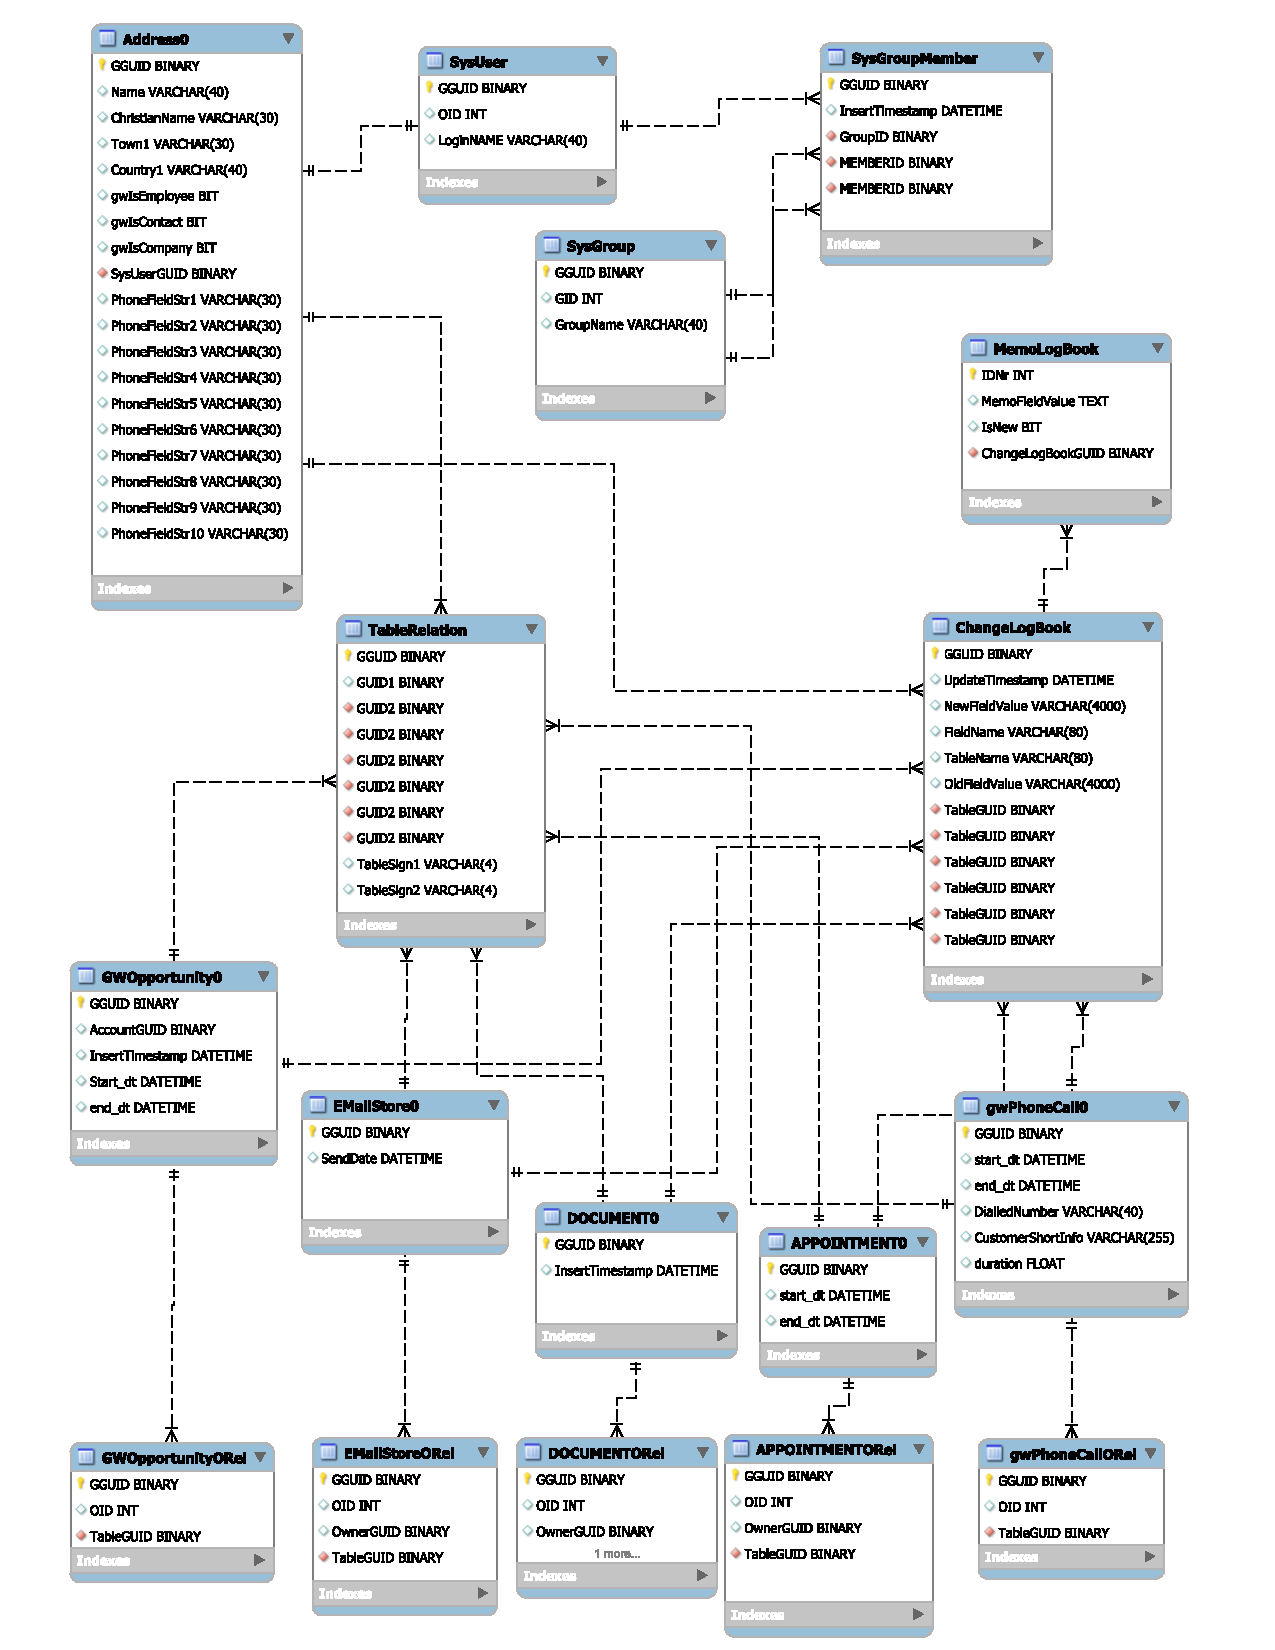
\includegraphics[width=1.0\textwidth]{pics/schema_alt.pdf}
	\caption{Auszug aus dem Schema des MSSQL 2008}
	\label{gw_schema_alt}
\end{figure}

Von den ursprünglich 398 Tabellen sind nur noch 17 übrig geblieben, auf die im Weiteren Verlauf eingegangen wird. Alle Tabellen enthalten in der ursprünglichen Form wesentlich mehr Spalten und wurden der Übersicht halber entfernt. Tabelle\textit{SysUser} besitzt drei Spalten, die von Bedeutung sind. Eine davon ist die \textit{GGUID}, die im folgenden nicht mehr erwähnt wird, da sie jede Tabelle enthält. Die \textit{OID} wird für jeden Nutzer einmalig vergeben und wird in anderen Tabellen als Zuordnungsmerkmal verwendet. \textit{LoginName} ist wie der Name schon sagt, der Benutzername des Nutzers und kann beim anmelden auf der Oberfläche, wieder verwendet werden. 

Aufgrund der Anforderung, Filterung durch Gruppen, wurden die Tabellen \textit{SysGroupMember} und \textit{SysGroup} hinzugezogen. \textit{SysGroup} besitzt eine \textit{GID}, die sich bei Gruppen genauso verhält, wie die \textit{OID} bei den Personen. Das Attribut \textit{GroupName}, wird für die Anzeige an der Oberfläche benötigt. Mithilfe dessen der Nutzer erkennen kann, welche Gruppe er gerade ausgewählt hat. \textit{SysGroupMember} stellt die Auflösungstabelle zwischen \textit{SysUser} und \textit{SysGroup} dar. Die Spalte \textit{GroupID} beinhaltet Werte aus der \textit{SysGroup-GGUID} Spalte. \textit{MemberID} folgt dem gleichen Ansatz, mit den \textit{SysUser-GGUID} Werten. In Hinsicht auf die Logikschicht, wird die Spalte \textit{InsertTimestamp} für Veränderungen innerhalb der Gruppen benötigt.

Die \textit{Adress0} Tabelle wird für die restlichen Filter Anforderungen benötigt. \textit{Town1} und \textit{Country1} geben die Stadt sowie das Land an, in der die Person ansässig ist. Zur Ermittlung, ob eine Person eine Kontaktperson, Mitarbeiter oder eine Firma repräsentiert, werden die Attribute \textit{gwIsContact}, \textit{gwIsEmployee} und \textit{gwIsCompany} benötigt. Name und \textit{ChristianName} beinhalten den Vor- und Nachname der Person, welche bei der Zuordnung der Ergebnisse an der Benutzeroberfläche hilfreich sind. Im voraus ist zu sagen, dass nicht alle Telefongespräche, über die dafür bestimmten Tabellen ermittelt werden können. Deswegen werden die Attribute \textit{PhoneFieldStr1-10} benötigt, mithilfe derer eine Zuordnung ermöglicht wird. 

Die \textit{TableRelation} enthält, wie in Abschnitt \ref{ch:Systemanalyse:sec:genesisWorld:subsec:db} behandelt, die Beziehungen der Datenbank. Auf das Szenario bezogen, wird für die \textit{GUID1} die \textit{GGUID} der \textit{SysUser} benutzt. Mithilfe der \textit{GUID2} könne,n die mit der Person verknüpften Termine, Verkaufschancen, Telefonate, Dokumente und E-Mails ermittelt werden. \textit{TableSign1} und \textit{TableSign2} werden zur Identifikation der jeweiligen Tabellen benötigt.

\textit{GWOpportunity0} enthält alle Informationen zu Verkaufschancen. Das Attribut \textit{InsertTimestamp} wird zur Feststellung des Erzeugungszeitpunktes benötigt. \textit{Start\_dt} und \textit{end\_dt} legen den Zeitraum der Verkaufschance fest. Der Besitzer einer Verkaufschance, wird über die \textit{AccountGUID} bestimmt. Mit \textit{EMailStore0}, \textit{Document0} \textit{Appointment0} und \textit{gwPhoneCall0} verhält es sich wie mit \textit{GWOpportunity0}. Bei \textit{EMailStore0} ist zu erwähnen, dass \textit{SendDate} zur zeitlichen Einordnung verwendet werden kann. Das Attribut \textit{DialledNumber} der Tabelle \textit{gwPhoneCall0}, wird zum Vergleich  mit der in der Adresse hinterlegten Telefonnummer, benötigt. Zur Überprüfung ob das Telefonat über einen Tag hinausging, wird das Attribut \textit{duration} herangezogen.

Bis jetzt galt die Annahme, dass alle Beziehungen über die\textit{TableRelation} bestimmt werden können. Dies trifft allerdings nicht für alle Beziehungen zu. Dort werden nur, die an der Oberfläche manuell verknüpften Tabellen aufbewahrt. Die restlichen Beziehungen können aus den ORel-Tabellen ermittelt werden. Jeder dieser Tabellen enthält eine \textit{OID} bzw. \textit{GID}, die zur Bestimmung der beteiligten Personen und/oder Gruppen dienen.

Eine Betrachtung basierend auf Zeitspannen, impliziert Veränderungen der Daten über die Zeit gesehen. Um diese Änderungen zu erfassen, wird die Tabelle \textit{ChangeLogBook} benötigt. \textit{NewFieldValue} enthält den neuen Wert eines Feldes. Wohingegen \textit{OldFieldValue} den alten Wert des Feldes enthält. Die Spalte des geänderten Wertes ist in \textit{FieldName} hinterlegt. Der Name der Tabelle, ist der Spalte \textit{TableName} zu entnehmen. Die Referenzierung auf eine Tupel wird in der Spalte \textit{TableGUID} vorgenommen. Aus Gründen des Speicherplatzverbrauchs werden nur varchar Datentypen bei Zeichenfolgen verwendet. Varchar ist jedoch auf 4000 Zeichen limitiert. Falls Zeichenfolgen diese Grenze überschreiten, werden die in der Tabelle \textit{MemoLogBook} abgelegt. Dort wird der Datentyp Text verwendet, der eine maximale Zeichenfolge von $2^{31-1}$  erlaubt.